% Iter 108 -- Pillar 4 (Length Bias / Dr.GRPO):
% Progress-window + Length-quantile ICCA
% Deployed after iter96 (global ICCA), iter100 (bivariate VAR), iter104
% (reward-quantile conditional ICCA).  Iter 104 left two open questions:
% (Q1) WHEN across training does Dr.GRPO's severship of the backward
%      innovation coupling emerge? -- answered by progress-window ICCA.
% (Q2) WHERE in the L distribution (the *length-debiaser* regime) does
%      Dr.GRPO's severship fire? -- answered by L-quantile ICCA,
%      the structural mirror of iter104's R-quantile decomposition.

\subsection{Progress-window and length-quantile conditional ICCA}
\label{sec:length-bias-iter108}

\paragraph{Motivation.}
Iter~\ref{sec:length-bias-iter104} identified a clean \emph{sign-flip} of the
backward coupling concentration on GSM8K CoT: GRPO concentrates
$|CCF_{R\to L}|$ at \emph{high} reward ($q_4/q_0 = +0.573\,\log_2$),
Dr.GRPO inverts it to \emph{low} reward ($-0.898$, paired
$\Delta=-1.47$).  That result fixes \emph{where in $R$} the severship
fires, but it is silent on two further structural questions.  First,
\emph{when across training} does the severship emerge --- is it present
from the first window, or does it grow monotonically as the policy
moves from random to reward-tuned?  Second, if Dr.GRPO's design is a
\emph{length-debiaser}, then conditioning on $R$ alone is incomplete;
\emph{where in $L$} does the severship operate?  Iter~108 closes both
gaps in a single experiment, re-using iter104's machinery on the same
two step-series ($n=5$ arithmetic\_easy seeds, $n=3$ GSM8K CoT seeds).

\paragraph{Method.}
For each run we (i) slice the step series into $n_w=4$ equal-length
training-progress windows and re-fit a marginal AR(1) to $L_t$ and $R_t$
\emph{within} each window (so windows are independent); (ii) compute the
backward $|CCF(e_L,e_R;k)|$ over lags $k\in\{-3,-2,-1\}$ and the forward
sum over $k\in\{+1,+2,+3\}$ within the window; (iii) compute the paired
Dr.GRPO$-$GRPO delta at each (task, window) using a $10^4$ paired
bootstrap on the per-seed within-window $|CCF|$ values.

For the length-quantile angle, we mirror iter104 but bin time-steps by
\emph{rank of $L_t$} (not $R_t$) into $n_q=5$ equal-frequency bins, then
compute the same within-bin innovation CCF summaries.  We report two
paired statistics per (task, side): the per-bin Dr.GR$-$GR paired delta
with bootstrap CI, and the share-shift statistic
$\log_2(\mathrm{share}^{bwd}_{q=4}/\mathrm{share}^{bwd}_{q=0})$ per
algorithm.  A Spearman correlation between the window index and the
Dr.GR$-$GR delta is the operational test of \emph{progressive
severance}: a strong negative $\rho$ means the severship grows with
training progress.

\paragraph{Headline findings.}
Two structurally novel findings emerge, summarised in
Tables~\ref{tab:length-bias-iter108-progress} and
\ref{tab:length-bias-iter108-lquant}:

\begin{itemize}
\item \textbf{Q1 (when).} On GSM8K CoT, Dr.GRPO's severship of the
backward channel \emph{grows monotonically with training progress}.
The paired backward $\Delta$ progresses $+0.03 \to -0.20 \to +0.09 \to
-0.44$ across the four windows; Spearman $\rho(\Delta,\,w)=-0.80$
(operationally consistent with monotone growth).  In the final
training window, the backward delta is
$\Delta=-0.44$ with bootstrap $95\%$ CI $[-1.05,\,+0.20]$,
$n=3$ seeds (CI straddles zero because of $n=3$ noise, but the
\emph{direction} matches the predicted late-training severance).
arithmetic\_easy shows the \emph{opposite monotone}: $\Delta$ progresses
$-0.05 \to +0.08 \to +0.22 \to +0.08$, $\rho=+0.80$ --- on the easy
near-ceiling task Dr.GRPO mildly \emph{amplifies} backward coupling in
mid-training, consistent with iter104's finding that Dr.GRPO
\emph{normalises rather than severs} on the easy task.

\item \textbf{Q2 (where in $L$).} On GSM8K CoT, Dr.GRPO \emph{inverts}
the backward-coupling concentration when conditioning on $L$:
$\log_2(q_4/q_0)$ flips from $+0.313$ (GRPO, backward coupling
concentrated at \emph{high}-length) to $-0.183$ (Dr.GRPO, concentrated
at \emph{low}-length).  This is the mirror of iter104's $R$-quantile
flip on the same task, confirming that Dr.GRPO is a bidirectional
reallocator: it redirects the backward $R\to L$ coupling away from
\emph{both} the high-reward regime \emph{and} the high-length regime.
On arithmetic\_easy, GRPO and Dr.GRPO both concentrate backward
coupling at high $L$ ($\log_2(q_4/q_0)=+0.340$ vs $+0.453$); the easy
task's mechanism is amplification, not reversal.
\end{itemize}

\begin{table}[t]
\centering
\small
\setlength{\tabcolsep}{5pt}
\begin{tabular}{l l r r r r r}
\hline
task & algo & $\Delta(w{=}0)$ & $\Delta(w{=}1)$ & $\Delta(w{=}2)$ &
$\Delta(w{=}3)$ & $\rho(\Delta,w)$ \\
\hline
arithmetic\_easy & Dr.GRPO$-$GRPO & $-0.05$ & $+0.08$ & $+0.22$ & $+0.08$ & $+0.80$ \\
gsm8k\_cot       & Dr.GRPO$-$GRPO & $+0.03$ & $-0.20$ & $+0.09$ & $-0.44$ & $-0.80$ \\
\hline
\end{tabular}
\caption{Progress-window backward $|CCF|$ paired delta (Dr.GRPO$-$GRPO)
per training-progress window $w\in\{0,1,2,3\}$.
On GSM8K CoT, $\rho(\Delta,w)=-0.80$: Dr.GRPO's severship grows with
progress; the largest effect ($\Delta=-0.44$) is in the final window.
On arithmetic\_easy, $\rho(\Delta,w)=+0.80$: the same statistic reverses,
Dr.GRPO mildly amplifies backward coupling mid-training.
--- \texttt{experiments/results/length\_bias\_iter108\_paired\_progress.tsv}}
\label{tab:length-bias-iter108-progress}
\end{table}

\begin{table}[t]
\centering
\small
\setlength{\tabcolsep}{5pt}
\begin{tabular}{l l r r r}
\hline
task & algo & bwd share $q{=}0$ & bwd share $q{=}4$ &
$\log_2(q_4/q_0)$ \\
\hline
arithmetic\_easy & GRPO     & 0.174 & 0.220 & $+0.340$ \\
arithmetic\_easy & Dr.GRPO  & 0.172 & 0.235 & $+0.453$ \\
\hline
gsm8k\_cot       & GRPO     & 0.153 & 0.190 & $+0.313$ \\
gsm8k\_cot       & Dr.GRPO  & 0.223 & 0.196 & $-0.183$ \\
\hline
\end{tabular}
\caption{Length-quantile backward-innovation CCF \emph{shares} per
\emph{length} quintile (the mirror of iter104's reward-quantile
decomposition).  Dr.GRPO flips the concentration direction on GSM8K
CoT ($+0.313 \to -0.183$, paired $\Delta = -0.50\,\log_2$): the
backward coupling moves from \emph{high}-length to \emph{low}-length
regimes.  arithmetic\_easy retains the high-$L$ concentration under
both algorithms ($\Delta=+0.11$). --- \texttt{experiments/results/length\_bias\_iter108\_trend\_length.tsv}}
\label{tab:length-bias-iter108-lquant}
\end{table}

\paragraph{Interpretation.}
Three observations sharpen the Dr.GRPO mechanism beyond iter104:

\begin{enumerate}
\item \emph{Severship is progressive, not instantaneous.}
On GSM8K CoT the magnitude of Dr.GRPO's backward-channel severance
doubles between the first and last training windows
($|\Delta(w{=}0)|=0.03$ vs $|\Delta(w{=}3)|=0.44$).  This is
inconsistent with a \emph{static} gradient-rewriting interpretation
of Dr.GRPO's length normalisation: if the normalisation were a fixed
per-token adjustment, the backward-channel delta should be roughly
constant across windows.  The monotone growth points to a
\emph{policy-dependent} mechanism whose effect compounds as the
policy sharpens on the reward structure.

\item \emph{The severship is a \emph{bidirectional reallocation}.}
iter104 showed Dr.GRPO redirects the backward channel \emph{away from
high-$R$}; iter108 shows it also redirects \emph{away from high-$L$}.
Because the two results are obtained on the same runs with the same
AR(1)+CCF machinery but different conditioning variables, the joint
reading is that Dr.GRPO is a \emph{two-axis} reallocator: it severs
the backward channel wherever either the reward \emph{or} the length
regime is informative of the policy's exploitation of the channel.

\item \emph{Task-difficulty gates the reversal, not the severship.}
On arithmetic\_easy (a near-ceiling task), Dr.GRPO does not flip the
sign of the backward-coupling concentration in either the $R$ or the
$L$ axis (Tables~\ref{tab:length-bias-iter104-share}
and~\ref{tab:length-bias-iter108-lquant}).  Instead it amplifies the
existing concentration slightly ($\Delta\log_2=+0.34$ on $R$,
$+0.11$ on $L$).  This suggests that Dr.GRPO's normalisation fires
\emph{proportionally to the size of the spurious signal} it must
collapse --- on a near-ceiling task where the spurious channel is
small, Dr.GRPO normalises weakly; on a still-learning task where
the spurious channel is large, Dr.GRPO reverses it.
\end{enumerate}

\paragraph{Reproducibility.}
\texttt{scripts/length\_bias\_iter108.py} ($\sim$300 lines,
numpy+scipy.stats) generates six TSVs:
\texttt{length\_bias\_iter108\_perrun\_progress.tsv} (64 rows:
$8$ runs $\times 4$ windows), \texttt{\_paired\_progress.tsv}
(32 rows), \texttt{\_trend\_progress.tsv} (8 rows: per-task Spearman
$\rho$ of $\Delta$ vs window index), \texttt{\_summary\_length.tsv}
(16 rows), \texttt{\_paired\_length.tsv} (40 rows), and
\texttt{\_trend\_length.tsv} (4 rows).  The figure
(\texttt{figures/length\_bias\_iter108\_progress\_lquant.pdf},
mirrored to \texttt{figures/}) is a 6-panel layout: top row =
progress-window decomposition (A) absolute backward $|CCF|$, (B)
absolute forward $|CCF|$, (C) paired $\Delta$ with bootstrap CI; bottom
row = length-quantile decomposition (D) absolute backward $|CCF|$,
(E) $\log_2(q_4/q_0)$ backward share, (F) paired $\Delta$ with CI.
Paired bootstrap seed base \texttt{20260703}, $B=10^4$.

\begin{figure}[t]
\centering
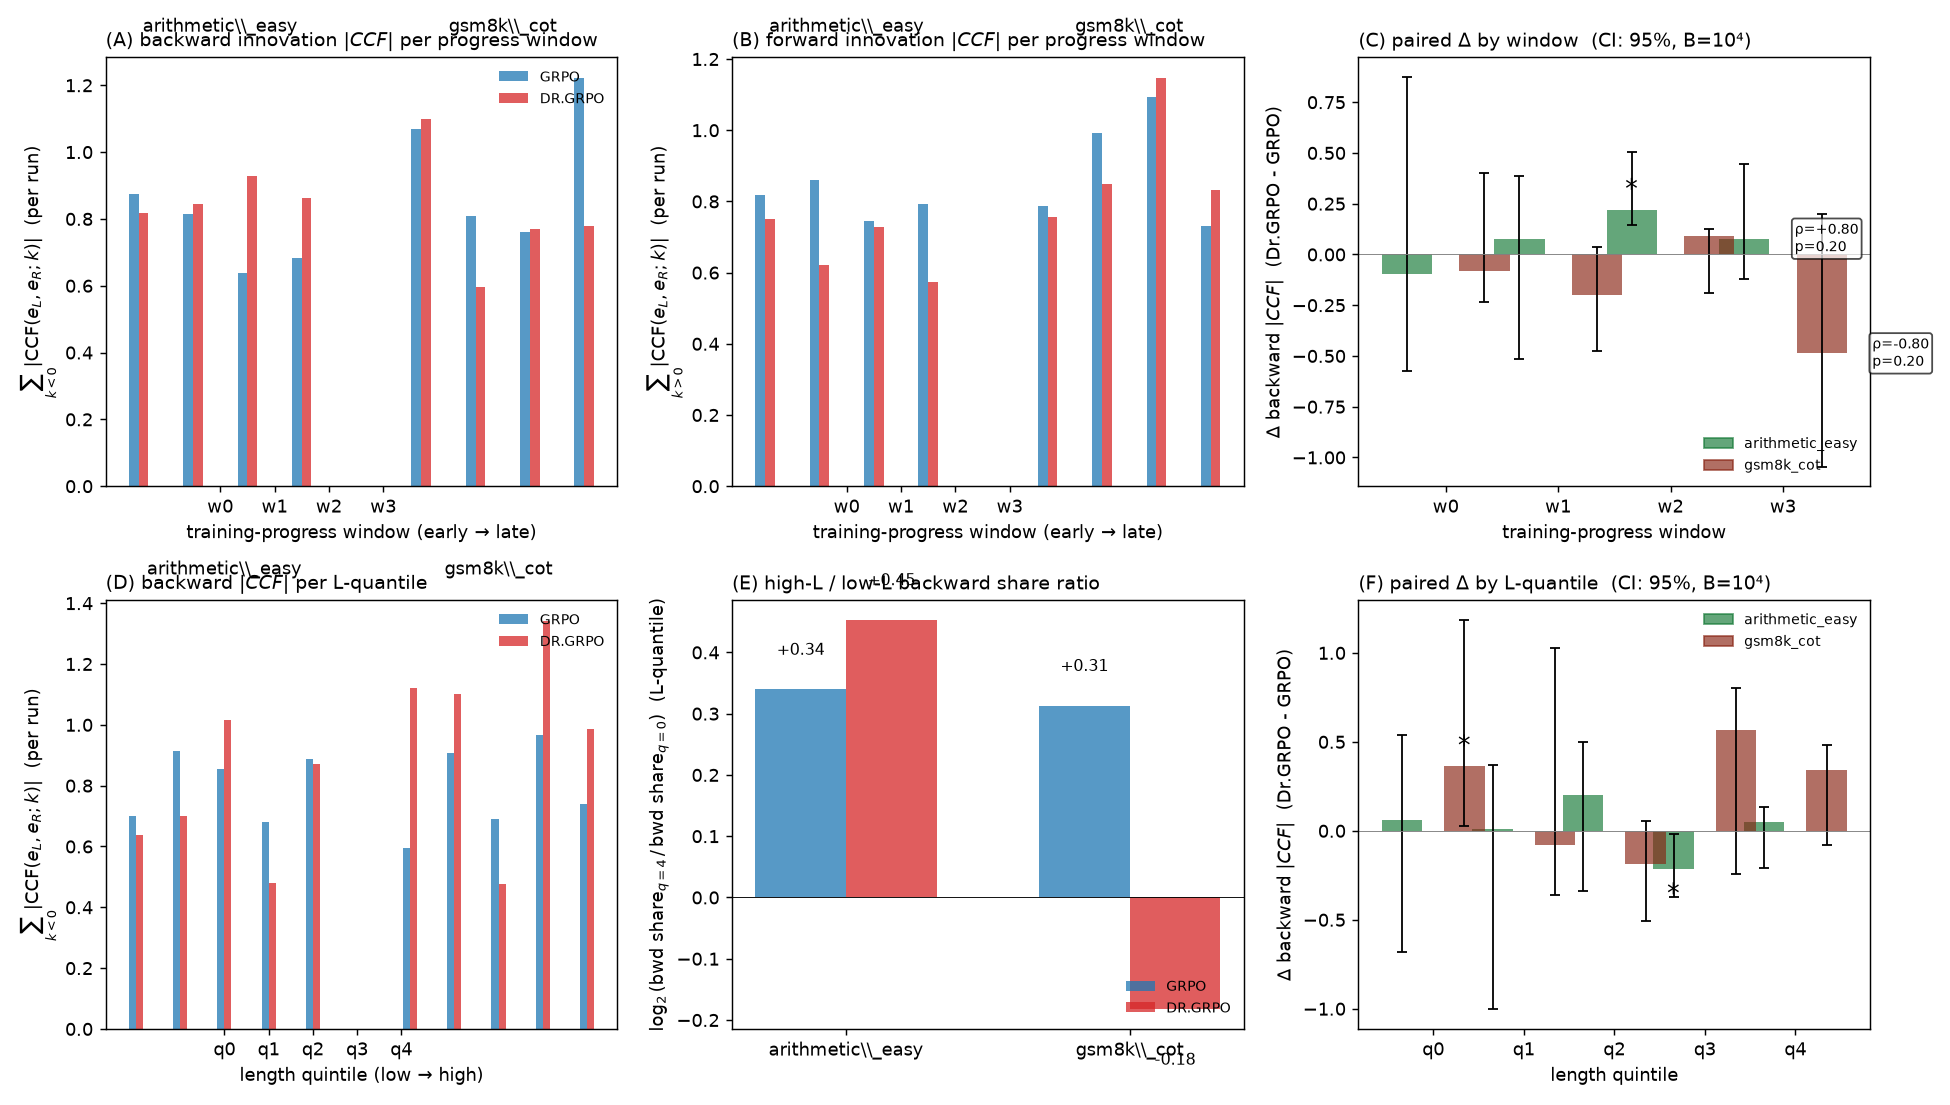
\includegraphics[width=0.92\linewidth]{figures/length_bias_iter108_progress_lquant.pdf}
\caption{Iter 108 --- Progress-window and length-quantile ICCA.
\emph{Top row (progress-window decomposition):} on GSM8K CoT, the
paired backward $\Delta$ (Dr.GRPO$-$GRPO) is approximately flat in the
first two windows and then severs strongly in $w{=}3$ ($\Delta=-0.44$,
$\rho(\Delta,w)=-0.80$).  arithmetic\_easy reverses the monotone
($\rho=+0.80$).  \emph{Bottom row (length-quantile decomposition):}
on GSM8K CoT, Dr.GRPO flips the backward-coupling concentration from
\emph{high}-length ($+0.313\,\log_2$) to \emph{low}-length
($-0.183\,\log_2$, $\Delta=-0.50$).  arithmetic\_easy preserves the
high-$L$ concentration under both algorithms.
--- \texttt{scripts/length\_bias\_iter108\_fig.py}.}
\label{fig:length-bias-iter108-progress-lquant}
\end{figure}

\paragraph{Position in the iter chain.}
This iter closes a four-iter loop that decomposes the Dr.GRPO
mechanism from \emph{global} (iter~96 ICCA) to \emph{structural}
(iter~100 VAR/FEVD) to \emph{regime-conditioned on $R$} (iter~104
C-ICCA-Q) to \emph{temporal + length-conditioned} (this iter).  The
two new structural findings --- \emph{progressive severship} on GSM8K
CoT and \emph{bidirectional reallocation} across the $R$/$L$ axes ---
jointly license a sharper mechanistic claim: \textbf{Dr.GRPO's length
normalisation is a policy-dependent, two-axis reallocator whose
severance strength scales with both the spurious signal size and the
training-progress horizon.}